\documentclass[final,t]{beamer}
\mode<presentation>
{
  \usetheme{I6dv}
}

\setbeamerfont{itemize}{size=\normalsize}
\setbeamerfont{itemize/enumerate body}{size=\normalsize}
\setbeamerfont{itemize/enumerate subbody}{size=\normalsize}

\setbeamertemplate{bibliography item}[text]

% additional packages
\usepackage{times}
\usepackage{amsmath,amsthm, amssymb, latexsym}
\usepackage{exscale}
\usepackage{booktabs, array}
\usepackage[english]{babel}
\usepackage[latin1]{inputenc}
\usepackage[orientation=landscape,size=a0,scale=1.22]{beamerposter}
\listfiles
\graphicspath{{figures/}}


\title{\Huge A View from the Hill: Where Cross Reality Meets Virtual Worlds}

\author[CJ Davies]{CJ Davies, Dr Alan Miller \& Dr Colin Allison}
\institute[University of St Andrews]{Open Virtual Worlds, School of Computer Science, University of St Andrews}
%\date[Feb. 1 , 2013]{Feb. 1 , 2013}

% abbreviations
\usepackage{xspace}
\makeatletter
\DeclareRobustCommand\onedot{\futurelet\@let@token\@onedot}
\def\@onedot{\ifx\@let@token.\else.\null\fi\xspace}
\def\eg{{e.g}\onedot} \def\Eg{{E.g}\onedot}
\def\ie{{i.e}\onedot} \def\Ie{{I.e}\onedot}
\def\cf{{c.f}\onedot} \def\Cf{{C.f}\onedot}
\def\etc{{etc}\onedot}
\def\vs{{vs}\onedot}
\def\wrt{w.r.t\onedot}
\def\dof{d.o.f\onedot}
\def\etal{{et al}\onedot}
\makeatother

\begin{document}
\begin{frame}
  \begin{columns}[t]
  
% ======= ======= ======= ======= ======= ======= =======
% left column
% ======= ======= ======= ======= ======= ======= =======

    \begin{column}{.31\linewidth}

		\begin{block}{Abstract}
			We present the \textbf{cross reality} system \textbf{Mirrorshades}, which enables users to be present and aware of both the real world and a virtual reality environment at the same time, along with a case study in the context of a cultural heritage application which enables users to compare a reconstruction of a 15th century chapel with its present day instantiation whilst walking through them.
		\end{block}

		\begin{block}{Explanation}
			Mirrorshades allows its user to observe and move around their Real World (RW) environment whilst wearing a wide field of view (FOV), stereoscopic 3D, Head Mounted Display (HMD) which allows them to alternatively view an immersive Virtual Reality (VR) environment from the equivalent vantage point. This is achieved by combining a head-tracked HMD, webcams, an indoor positioning system (IPS) and a 3D game engine, into a mobile cross reality (XR) platform.
						
						
			\begin{figure}[h]
				\begin{center}
					\includegraphics[width=\linewidth]{images/experiment_picture_2.png}

					\textit{A user study of Mirrorshades under way in an important cultural heritage site.}
				\end{center}
			\end{figure}
					
		\end{block}

		\begin{block}{Position of Cross Reality}
			The relationship between XR and other alternate realities can be visualised using Milgram and Kishino's virtuality continuum, that stretches from an entirely real environment at one extreme to an ontologically parallel but entirely virtual environment at the other. A defining feature of XR is that it features two discrete environments, one real and the other virtual, each complete unto itself. This distinguishes XR from augmented reality, where a single mixed reality environment is created by the overlay of virtual content atop a view of the real.	
			
			\begin{figure}[h]
				\begin{center}
					\includegraphics[width=\linewidth]{images/virtuality-continuum-cross-reality-1.png}

					\textit{The two constituent environments of an XR system (circled).}
				\end{center}
			\end{figure}		
			
		\end{block}

  \end{column}

% ======= ======= ======= ======= ======= ======= =======
% middle column
% ======= ======= ======= ======= ======= ======= ======= 
    
    \begin{column}{.31\linewidth}

		\begin{block}{Design of Mirrorshades Platform}
			\begin{columns}
				\begin{column}{.45\linewidth}
					\begin{figure}[h]
				\begin{center}
					\includegraphics[width=\linewidth]{images/system-architecture.png}
					
					\textit{High level architectural overview of Mirrorshades platform.}
				\end{center}
			\end{figure}
				\end{column}
				
				\begin{column}{.45\linewidth}
					The platform displays both real and virtual feeds from the mobile client to the user in stereoscopic 3D, tracking their head movements such that the virtual feed can be adjusted appropriately and  tracking their location to move the position of their virtual proxy accordingly. User input from a controller is used to trigger transitions between real and virtual visual feeds.				
				\end{column}		
			\end{columns}
		\end{block}

		\begin{block}{Implementation of Mirrorshades Platform}
			\begin{figure}[h]
				\begin{center}
					\includegraphics[width=\linewidth]{images/experimental-implementation.png}

					\textit{Implementation of the Mirrorshades platform.}
				\end{center}
			\end{figure}

			Our implementation comprises;
			\begin{itemize}
				\item an Oculus Rift DK1 HMD with a stereo camera solution that provides approximately 87 degrees horizontal FOV of the RW environment;
				\item a USB battery pack, to power the HMD;
				\item a laptop computer, with Intel i7 processor and Nvidia GT 650M graphics;
				\item an Android smartphone, running Android 4.4.4;
				\item an Xbox 360 wireless controller, with USB receiver.
			\end{itemize}
			
			\begin{columns}
				\begin{column}{.45\linewidth}
					\begin{figure}[h]
						\begin{center}
							\includegraphics[width=\linewidth]{images/rift.jpg}
							
							\textit{Oculus Rift DK1 with stereo camera solution.}
						\end{center}
					\end{figure}
				\end{column}
				
				\begin{column}{.45\linewidth}
					The novel aspect of the platform is the ability it imparts upon its user to visually transition between equivalent vantage points in RW and VR environments. In order to achieve the highest quality of experience with this system, it is vital to determine how best to implement these transitions and as such multiple different transition styles have been implemented, including those controlled by the user and those outwith their control.
					
					%The novel aspect of this platform is the ability it imparts upon its user to switch their locus of attention between equivalent vantage points in RW and VR environments whilst walking around. This is achieved by the user performing transitions between RW visual stimuli and VR visual stimuli, both presented via their HMD. This extends existing XR research by allowing the user to engage with the visual stimuli of the VR component of a XR system from any position and at any time.
				\end{column}
			\end{columns}
			
			
		\end{block}
				
    \end{column}
    
% ======= ======= ======= ======= ======= ======= =======
% right column
% ======= ======= ======= ======= ======= ======= =======    
    
    \begin{column}{.31\linewidth}
    
    	\begin{block}{Case Study - Cultural Heritage}
    		Cultural heritage has seen widespread application of both AR and VR. AR has been used to add artefacts, actors and reconstructed architecture to views of present day sites that bear traces of their original status, whilst VR has been used to host more complete reconstructions of entire buildings and settlements for interaction via screen, HMD and CAVE.

    		\begin{figure}[h]
				\begin{center}
					\includegraphics[width=\linewidth]{images/sallies_colour.png}
					%\caption{The virtual reconstruction of St Salvator's chapel.}
					
					\textit{Virtual reconstruction of St Salvator's chapel in St Andrews.}
				\end{center}
			\end{figure}
    		
    		
		\end{block}

		\begin{block}{St Salvator's Chapel}
			Founded in 1450 but stripped of its medieval fittings during the Protestant Reformation (1517-1648), St Salvator's chapel in St Andrews looks markedly different today than it did upon its completion. An existing VR reconstruction of the chapel as it stood in 1450 and the marked differences between the current and VR buildings made it an ideal candidate for investigation into mobile XR with the Mirrorshades platform.
			
			\vspace{2mm}
			
			\begin{figure}[h]
				\begin{center}
					%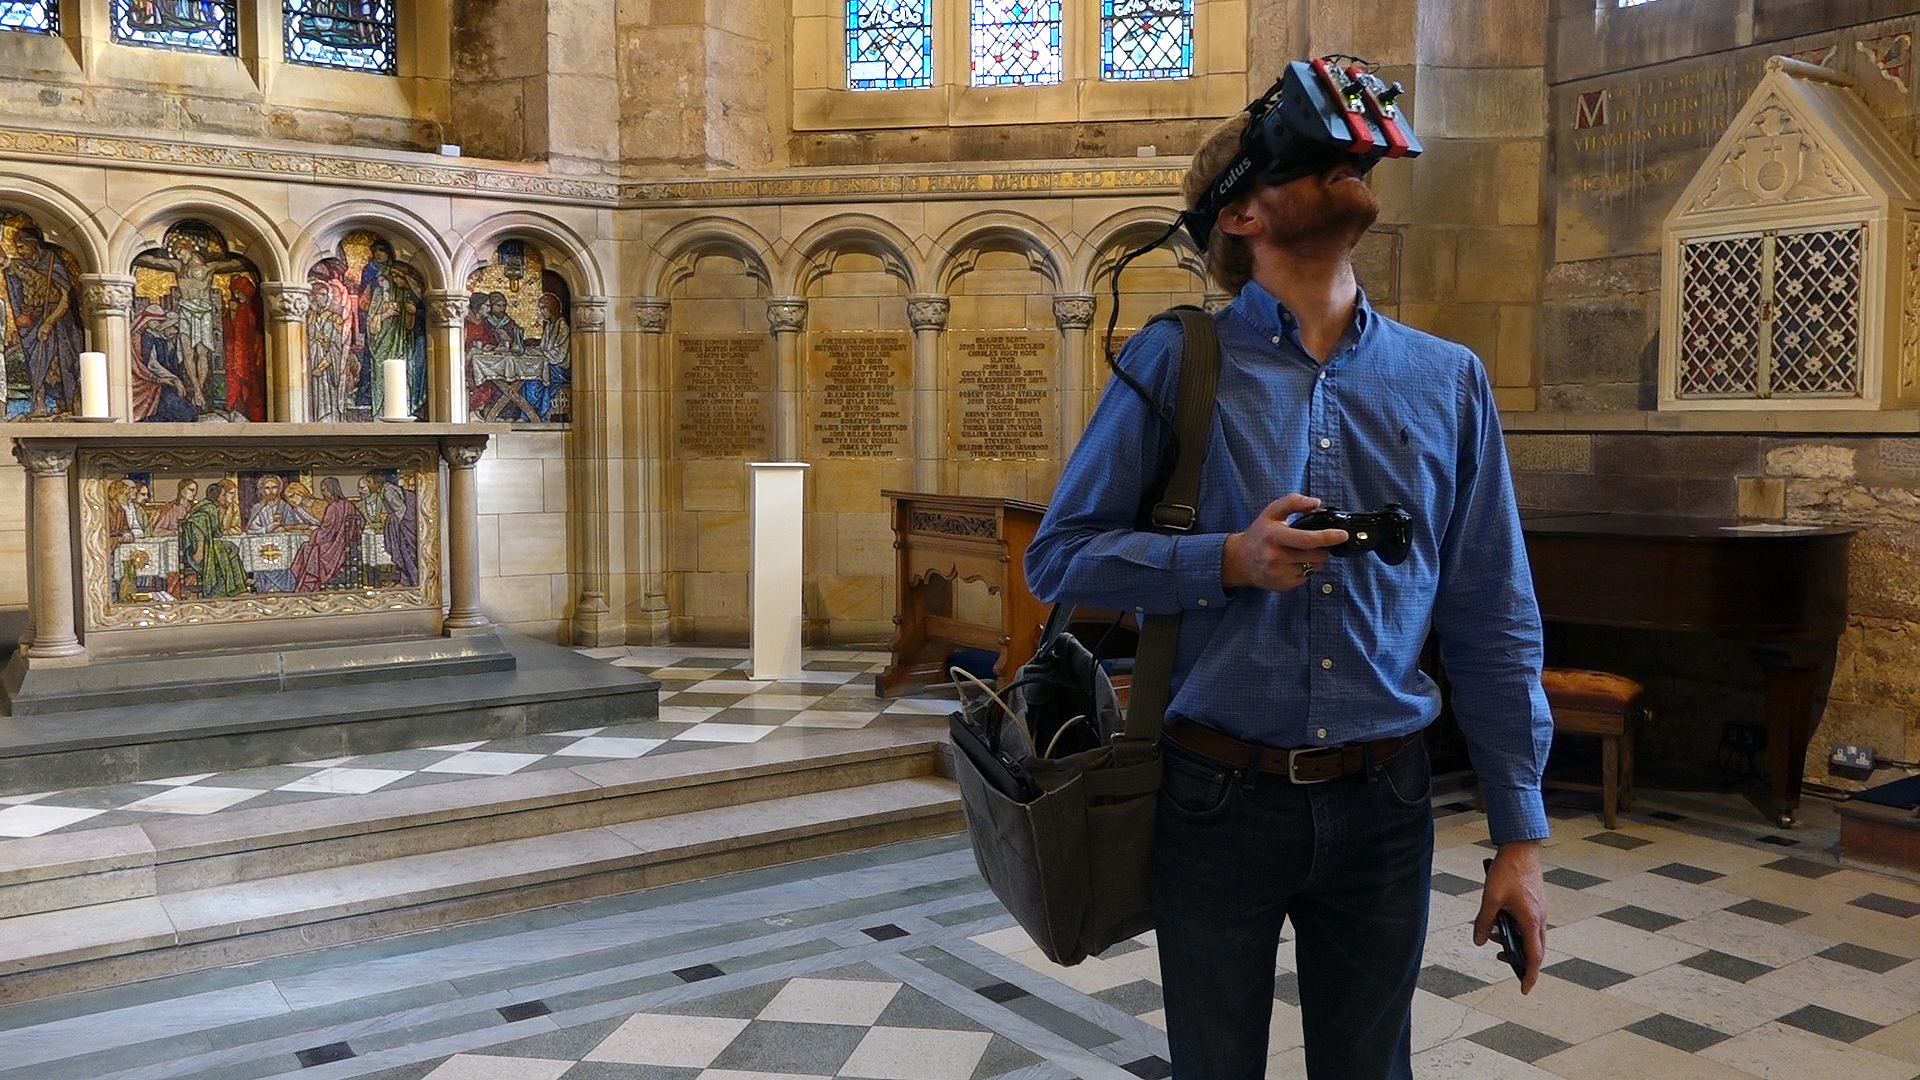
\includegraphics[width=\linewidth]{images/experiment_picture.png}
					\includegraphics[width=\linewidth]{images/experiment_picture_dual.png}
					
					\textit{A user during a study remarking upon a past feature in the virtual reconstruction of St Salvator's chapel that is substantially relocated today.}
				\end{center}
			\end{figure}
		\end{block}
	       	
		\begin{block}{Future Work}
			Evaluation of user studies in St Salvator's chapel is under way, assessing responses to the Mirrorshades platform in comparison to a traditional static VR experience and assessing reactions to/preferences toward the different styles of transition between real and virtual environments provided.

		\end{block}
    
	\end{column}
    
  \end{columns}
 
\end{frame}

\end{document}